% !TEX root = ../ac_paper.tex

\section{Stable Andrews-Curtis Conjecture and Unknot Diagrams}

\subsection{Stable AC conjecture}

The stable Andrews--Curtis conjecture, also called the weak Andrews--Curtis conjecture in the literature, see e.g. \cite{MMS,Meier2016,Bagherifard2021}, allows for two additional moves in addition to the usual AC-moves:
\begin{enumerate}[label=(AC\arabic*)]
	\setcounter{enumi}{3}
	\item Include a new generator and a trivial relator, i.e. replace $\angles{x_1, \dots, x_n \mid r_1, \dots, r_n}$ by $\angles{x_1, \dots, x_n, x_{n+1} \mid r_1, \dots, r_n, x_{n+1}}$.
	\item Remove a trivial relator and the corresponding generator, i.e. the inverse of (AC4).
\end{enumerate}

\begin{definition}
If two balanced presentations of the trivial group are related by a sequence of AC-transformations (AC1) through (AC5), we say that they are \textit{stably AC-equivalent}.
\end{definition}
The stable Andrews--Curtis conjecture states that any balanced presentation is stably AC-equivalent to the trivial presentation.

It is useful to note that these moves allow us to reduce presentations of the trivial group in the following way: by substituting an equivalent expression of a generator into all relators and then removing that generator entirely.
\begin{lemma}[Substitution]
    \label{lem:substitution}
    Let $P=\langle x_1,\cdots, x_n, y \mid r_1,\cdots, r_n, y^{-1}w\rangle$ be a presentation of the trivial group, where $w$ is a word in $x_1,\ldots,x_n$. Then $P'=\langle x_1,\cdots, x_n \mid r_1',\cdots, r_n'\rangle$ is stably AC-equivalent to $P$, where $r_i'$ is $r_i$ with all occurrences of $y$ replaced by $w$.
\end{lemma}
\begin{proof}
    First, we can use (AC1)–(AC3) to iteratively replace every occurrence of $y$ in $r_1,\cdots,r_n$ with $w$, giving $\widetilde{P}=\langle x_1,\cdots,x_n,y\mid r_1',\cdots,r_n',y^{-1}w\rangle$. Since $r_1',\cdots,r_n'$ contain no $y$, we can define the surjective homomorphism $\phi:\widetilde{P}\longrightarrow P'$ by $\phi(x_i)=x_i$ and $\phi(y)=w$. Since $\widetilde{P}$ is trivial, $P'$ is trivial. Therefore, the normal closure of $r_1',\cdots, r_n'$ gives the free group generated by $x_1,\cdots, x_n$, which means $w$ can be written as a product of conjugates of the $r_i$, namely, $w=w_1 (r_{i_1}')^{\pm1}w_1^{-1}w_2 (r_{i_2}')^{\pm 1}w_2^{-1}\cdots w_m (r_{i_m}')^{\pm 1}w_m^{-1}$, for words $w_i$ in the $x_i$ and $i_k \in \{1,\ldots,n\}$. Note $m$ may be much larger than $n$. Now using (AC1)–(AC3) we can transform  $y^{-1}w$ to $w_1 (r_{i_1}')^{\pm1}w_1^{-1}\cdots w_m (r_{i_m}')^{\pm 1}w_m^{-1}w^{-1}y$ which equals $y$, and then we can remove $y$ by (AC5).
\end{proof}

\subsection{Unknot diagrams}

One way to generate interesting presentations that are stably AC-trivial is through diagrams on the unknot. Since the knot group of the unknot is the infinite cyclic group $\mathbb{Z}$, adding any relator with exponent sum $\pm 1$ will give us a presentation of the trivial group. Moreover, Reidemeister moves can be realized by (AC1)–(AC5), so any such balanced presentation will be stably AC-trivial. Using the Wirtinger presentation of the knot group allows us generate many such examples, which we can summarize in the following prop:

\begin{proposition}\label{prop:unknot}
    Let $\langle x_1,\cdots, x_n\, |\, r_1, \cdots, r_n \rangle$ be the Wirtinger presentation of an unknot diagram. Then for any $k=1,\ldots,n$ and word $w$ in the $x_i$ with exponent sum $\pm 1$, the balanced presentation of the trivial group $\langle x_1,\cdots, x_n\,|\, r_1,\cdots, r_{k-1}, r_{k+1},\cdots, r_n, w\rangle$ is stably Andrews-Curtis-trivial.
\end{proposition}
\begin{remark}
The method to construct stably AC-trivial balanced presentations from unknot diagrams was introduced in \cite{MMS}.  We formulate Proposition~\ref{prop:unknot} for self-containment and prove it in this section.
\end{remark}

\subsubsection{Wirtinger presentations of an unknot diagram}
We briefly recall the Wirtinger presentation of a knot group. Given any oriented knot diagram with $n$ crossings, we assign generators $\{x_i\}_{i=1}^n$ to each of the arcs, and each crossing gives us a relator $\{r_i\}_{i=1}^n$. In our notation, the left crossing in Figure~\ref{fig:wp} corresponds to the relator $y=x^{-1}zx$ and the right one gives $y=xzx^{-1}$.

\begin{figure}
    \centering
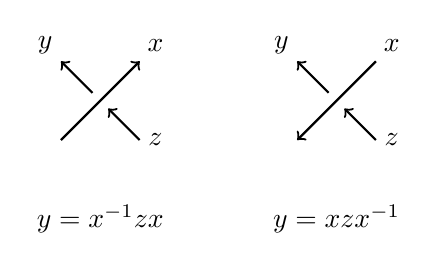
\begin{tikzpicture}
\draw[thick,->] (0,0)--(1,1);
\draw[thick,->] (1,0)--(0.6,0.4);
\draw[thick,->] (0.4,0.6)--(0,1);
\node at (1.2,1.2){$x$};
\node at (-0.2,1.2){$y$};
\node at (1.2,0){$z$};
\node at (0.5,-1){$y=x^{-1}zx$};

\draw[thick,->] (4,1)--(3,0);
\draw[thick,->] (4,0)--(3.6,0.4);
\draw[thick,->] (3.4,0.6)--(3,1);
\node at (4.2,1.2){$x$};
\node at (2.8,1.2){$y$};
\node at (4.2,0){$z$};
\node at (3.5,-1){$y=xzx^{-1}$};

\end{tikzpicture}
    \caption{Types of Crossings}
    \label{fig:wp}
\end{figure}
These generators and relators form a balanced presentation of the fundamental group of the knot complement. Moreover, there exists an ordering of the relators and a choice of $\pm 1$ as exponents such that the relators satisfy the equation
$$\prod_{i=1}^nr_i^{\pm1}=1.
$$
Thus any relator $r_k$ can be eliminated, giving $\langle x_1,\cdots,x_n\mid r_1,\cdots,r_{k-1},r_{k+1},\cdots,r_n\rangle$, without changing the underlying group. When the knot is an unknot, the fundamental group of the knot complement is $\mathbb{Z}$, which can be generated by any generator $x_i$. So after adding a relator $w$ which is any word in $x_1,\ldots,x_n$ with exponent sum $\pm1$, we get a balanced presentation $\langle x_1,\cdots,x_n\mid r_1,\cdots,r_{k-1},r_{k+1},\cdots,r_n,w\rangle$ of the trivial group as in \textbf{Proposition~\ref{prop:unknot}}.

\subsubsection{Reidemeister moves are stable Andrews-Curtis moves} Two diagrams of the same knot can be related by a finite sequence of the three
Reidemeister moves in Figure \ref{fig:rm}. Here we distinguish \textbf{R2a} and \textbf{R2b} just because they give slightly different computation about the presentations. First described in \cite{WADA1994241}, Reidemeister moves can be realized by (AC1)–(AC5). We list the correspondence between Reidemeister moves and (AC1)–(AC5) as follows for self-containment. We consider the presentations obtained from Wirtinger presentations of any unknot diagram by eliminating one arbitrary relator and adding one relator $w$ which is any word in the generators with exponent sum $\pm1$, as described in the previous subsection. Since we want to consider their behavior under Reidemeister moves, we can assume that the relator eliminated is not one given by the crossings in \textbf{R1}, \textbf{R2a}, \textbf{R2b}, \textbf{R3}. We note, however, that since any relator in a Wirtinger presentation can be written as the product of the other relators, the relator we eliminated can be recovered using (AC1)–(AC3).
\\
\\
\textbf{R1}:
\begin{align*}
\langle x_1,\cdots,x_n,x,y\mid r_1,\cdots,r_n,yx^{-1},w\rangle\longleftrightarrow\langle x_1,\cdots,x_n,x\mid r_1',\cdots,r_n',w'\rangle
\end{align*}
Here $r_i'$ and $w'$ are obtained from replacing $y$ in $r_i$ and $w$ by $x$. The equivalence comes from the substitution in \textbf{Lemma~\ref{lem:substitution}}.
\\
\\
\textbf{R2a}:
\begin{align*}
\,\,&\langle x_1,\cdots,x_n,x,y,z,u\mid r_1,\cdots,r_{n+1},xyz^{-1}y^{-1},zy^{-1}u^{-1}y,w\rangle
\\
&\longleftrightarrow\langle x_1,\cdots,x_n,x,y,u\mid r_1',\cdots,r_{n+1}',ux^{-1},w'\rangle
\\
&=\langle x_1,\cdots,x_n,x,y,u\mid r_1,\cdots,r_{n+1},ux^{-1},w'\rangle
\\
&\longleftrightarrow\langle x_1,\cdots,x_n,x,y\mid \tilde{r}_1,\cdots,\tilde{r}_{n+1},\tilde{w}\rangle
\end{align*}
Here $r_i',w'$ are obtained from replacing $z$ in $r_i,w$ by $y^{-1}xy$; $\tilde{r_i}$ from replacing $u$ in $r_i$ by $x$; and $\tilde{w}$ from replacing $u$ in $w'$ by $x$. The second equation comes from the fact that the $r_i$ do not contain $z$.
\\
\textbf{R2b} is similar to \textbf{R2a}.
\\
\\
\textbf{R3}:
\begin{align*}
&\langle x_1,\cdots,x_n,x,y,z,u,v,r\mid r_1,\cdots,r_{n+2},vxy^{-1}x^{-1},urv^{-1}r^{-1},rxz^{-1}x^{-1},w\rangle
\\
&\longleftrightarrow\langle x_1,\cdots,x_n,x,y,z,u,r\mid r_1,\cdots,r_{n+2},urxy^{-1}x^{-1}r^{-1},rxz^{-1}x^{-1},w'\rangle
\\
&\longleftrightarrow\langle x_1,\cdots,x_n,x,y,z,u,r\mid r_1,\cdots,r_{n+2},uxzy^{-1}z^{-1}x^{-1},rxz^{-1}x^{-1},w'\rangle
\\
&\longleftrightarrow\langle x_1,\cdots,x_n,x,y,z,u,r,t\mid r_1,\cdots,r_{n+2},uxzy^{-1}z^{-1}x^{-1},rxz^{-1}x^{-1},tzy^{-1}z^{-1},w'\rangle
\\
&\longleftrightarrow\langle x_1,\cdots,x_n,x,y,z,u,r,t\mid r_1,\cdots,r_{n+2},rxz^{-1}x^{-1},tzy^{-1}z^{-1},uxt^{-1}x^{-1},w'\rangle
\end{align*}
Here $w'$ is obtained from replacing $v$ in $w$ by $xyx^{-1}$.


After reducing our diagram to the trivial diagram of the unknot, we are left with $\langle x \mid \bar w\rangle$, where $\bar w$ is $w$ after applying all the Reidemeister moves. This is because the trivial diagram of the unknot gives the presentation $\langle x\mid \,\,\rangle$ of the infinite cyclic group, so $\bar w$ is the only relator remaining.  Moreover, $\bar w = x^{\pm1}$ since at each stage, $w$ has exponent sum $\pm 1$, so $\langle x \mid \bar w\rangle$ can be reduced to the trivial presentation $\langle \,\, \mid \,\, \rangle$. Thus \textbf{Proposition \ref{prop:unknot}} is proven.

\begin{figure}
    \centering
\begin{tikzpicture}
\draw[thick,rounded corners] (0,0)--(2,0)--(2,-1)--(1,-1)--(1,-0.2);
\draw[thick,rounded corners] (1,0.2)--(1,1);

\draw[<->] (2.5,0)--(3.5,0);

\draw[thick,rounded corners] (4,0)--(5,0)--(5,1);

\node at (4.5,-0.5){$x$};
\node at (0.5,-0.5){$x$};
\node at (1.5,0.5){$y$};

\node at (0.5,0){$>$};
\node at (1,0.5){\rotatebox{90}{$>$}};
\node at (4.5,0){$>$};

\node at (-0.5,0){\textbf{R1}};

\node at (7.5,-3){\textbf{R2b}};

\draw[thick] (9,-2)--(9,-2.3);
\draw[thick] (9,-2.7)--(9,-3.3);
\draw[thick] (9,-3.7)--(9,-4);

\draw[thick,rounded corners] (10,-2)--(10,-2.5)--(8.5,-2.5)--(8.5,-3.5)--(10,-3.5)--(10,-4);

\node at (9,-1.7){$x$};
\node at (10,-1.7){$y$};
\node at (9.2,-3){$z$};
\node at (9,-4.3){$u$};

\node at (9,-2){\rotatebox{90}{$>$}};
\node at (10,-2){\rotatebox{90}{$>$}};
\node at (9,-3){\rotatebox{90}{$>$}};
\node at (9,-3.7){\rotatebox{90}{$>$}};

\draw[<->] (10.5,-3)--(11.5,-3);

\draw[thick] (12.5,-2)--(12.5,-4);
\draw[thick] (13.5,-2)--(13.5,-4);

\node at (12.5,-3){\rotatebox{90}{$>$}};
\node at (13.5,-3){\rotatebox{90}{$>$}};

\node at (12.5,-1.7){$x$};
\node at (13.5,-1.7){$y$};

\draw[thick] (1,-2)--(1,-2.3);
\draw[thick] (1,-2.7)--(1,-3.3);
\draw[thick] (1,-3.7)--(1,-4);

\draw[thick,rounded corners] (2,-2)--(2,-2.5)--(0.5,-2.5)--(0.5,-3.5)--(2,-3.5)--(2,-4);

\node at (1,-2){\rotatebox{90}{$>$}};
\node at (2,-2.3){\rotatebox{90}{$<$}};
\node at (1,-3){\rotatebox{90}{$>$}};
\node at (1,-3.7){\rotatebox{90}{$>$}};

\draw[<->] (2.5,-3)--(3.5,-3);

\draw[thick] (4.5,-2)--(4.5,-4);
\draw[thick] (5.5,-2)--(5.5,-4);

\node at (4.5,-3){\rotatebox{90}{$>$}};
\node at (5.5,-3){\rotatebox{90}{$<$}};

\node at (4.5,-1.7){$x$};
\node at (5.5,-1.7){$y$};

\node at (1,-1.7){$x$};
\node at (2,-1.7){$y$};
\node at (1.2,-3){$z$};
\node at (1,-4.3){$u$};

\node at (-0.5,-3){\textbf{R2a}};

\draw[thick] (1,-5)--(1,-8);
\draw[thick] (0.5,-7.5)--(0.8,-7.5);
\draw[thick,rounded corners] (1.2,-7.5)--(2,-7.5)--(2,-5.5)--(3.5,-5.5);
\draw[thick] (0.5,-6.5)--(0.8,-6.5);
\draw[thick] (1.2,-6.5)--(1.8,-6.5);
\draw[thick] (2.2,-6.5)--(3.5,-6.5);

\draw[<->] (4,-6.5)--(5,-6.5);

\draw[thick] (5.5,-6.5)--(6.8,-6.5);
\draw[thick,rounded corners] (5.5,-7.5)--(7,-7.5)--(7,-5.5)--(7.8,-5.5);
\draw[thick,rounded corners] (7.2,-6.5)--(7.8,-6.5);
\draw[thick] (8,-5)--(8,-8);
\draw[thick] (8.2,-5.5)--(8.5,-5.5);
\draw[thick] (8.2,-6.5)--(8.5,-6.5);

\node at (0.5,-5.5){$x$};
\node at (0.5,-6.2){$y$};
\node at (0.5,-7.2){$z$};
\node at (3,-5.2){$r$};
\node at (3,-6.2){$u$};
\node at (1.5,-6.2){$v$};

\node at (1,-5.5){\rotatebox{90}{$>$}};
\node at (0.7,-6.5){$>$};
\node at (0.7,-7.5){$>$};
\node at (1.5,-6.5){$>$};
\node at (3,-5.5){$>$};
\node at (3,-6.5){$>$};

\node at (8,-4.5){$x$};
\node at (6,-6.2){$y$};
\node at (6,-7.2){$z$};
\node at (9,-5.5){$r$};
\node at (9,-6.5){$u$};
\node at (7.5,-6.2){$t$};

\node at (8,-5){\rotatebox{90}{$>$}};
\node at (6,-6.5){$>$};
\node at (6,-7.5){$>$};
\node at (8.5,-6.5){$>$};
\node at (8.5,-5.5){$>$};
\node at (7.5,-6.5){$>$};

\node at (-0.5,-6){\textbf{R3}};

\end{tikzpicture}
    \caption{Reidemeister moves}
    \label{fig:rm}
\end{figure}


\subsubsection{Constructing Infinite Familes}
Any diagram of the unknot with $n$ crossings gives us $n$ examples of infinite families of presentations that are known to be stably AC-trivial, as given by the proposition.

Moreover, we can use stable AC-moves, especially the substitution move in Lemma~\ref{lem:substitution}, to reduce the number of generators and relations in these families of presentations. Indeed, if we restrict our attention to the relators coming from the Wirtinger presentation (i.e., without changing the free choice of $w$), we can get similar infinite families of presentations with fewer generators. This is valuable since most of the focus in studying the (stable) Andrews-Curtis conjecture is given to presentations with a small number of generators, especially 2 and 3.

\begin{remark}
This approach can at best generate interesting infinite families with three generators and relators, since removing $w$ will always give us a presentation of $\mathbb{Z}$ and so any two-generator presentation must be just $\langle x,y \mid x=\pm y, w\rangle$.
\end{remark}
\begin{remark}
    Each infinite family coming from Proposition~\ref{prop:unknot} will give many distinct infinite families with fewer generators, as we have many different ways to simplify the groups that lead to different presentations.
\end{remark}
\begin{remark}
    In order to get interesting examples, it seems sensible to look at hard unknot diagrams, as the easier it is to change the diagram into the trivial diagram of the unknot, the easier it should be for the computer algorithms to trivialize the resulting presentations.
\end{remark}
\begin{remark}
    On the other hand, the more complicated the knot diagram, the harder it will be to simplify the presentation down to three generators, and the less likely such a presentation is of reasonable length.
\end{remark}
\begin{remark}
    We can also make presentations more complicated by choosing simplification steps that make the presentation more complicated. However it seems more likely to get interesting presentations from choosing a complicated knot diagram and simplifying more.
\end{remark}

\begin{conjecture}
    Every stably AC-trivial presentation of the form from Proposition~\ref{prop:unknot} can also be stably AC-trivialized without (AC4), and in particular by just doing substitutions.
\end{conjecture}

Note that realizing Reidemeister moves with stable AC moves \emph{does} require (AC4), and thus this conjecture is not a consequence of the proof of the proposition. We checked that it holds in many of hard unknot diagrams in \cite{burton2021harddiagramsunknot}, in particular for the Culprit, D28, Goeritz, Ochai I, and Tuzun Sikora.

If true, it provides some evidence against this approach generating lots of interesting examples of stably AC-trivial presentations.
\subsubsection{Examples}
One famous hard unknot diagram is the 10-crossing Culprit, first introduced in \cite{kauffman2014hardunknotscollapsingtangles}. One possibly interesting infinite family coming from this diagram is the following:
\begin{proposition}
    Any presentation of the form
    \[
\langle x,y,z \,\mid \, xzxz^{-1}x^{-1}yzyz^{-1}y^{-1}z^{-1}y^{-1}, zx^{-1}yzy^{-1}z^{-1}y^{-1}x, w \rangle,
\] where $w$ is a word with exponent sum $\pm 1$, is a stably AC-trivial presentation of the trivial group. [is it worth showing the substitution steps of how you get this presentation from the culprit?]
\end{proposition}
However, it is difficult to find a choice of $w$ that gives any non-trivial result. For example, if $w=z^{-1}w'$, where $w'$ is a word in $x$ and $y$ of length $\leq 8$, then the greedy search is able to instantly trivialize the presentation.